%%% XeLaTeX-article %%%
%# -*- coding: utf-8 -*-
%!TEX encoding = UTF-8 Unicode
%!TEX TS-program = xelatex  
%---------------------虽然加了%还是要保留!

\documentclass[17pt]{beamer}
\mode<presentation>
{
\usetheme[width=40pt]{Hannover}
\usecolortheme[]{dove}
\usefonttheme[]{structurebold}
\setbeameroption{hide notes}
}

\usepackage{fontspec}
\setmainfont{Arial} %设置主字体
\newfontfamily\sanskritfont[Script=Devanagari,Mapping=romantodevanagari,Scale=1.15]{Sanskrit 2003}             %输出天城体
%\newfontfamily\sanskritfont[Mapping=tex-text]{Times New Roman}              %输出转写
\doublehyphendemerits=-10000
\newcommand{\skt}[1]{{\sanskritfont{#1}}} %输出天城体
\newcommand{\skttrans}[1]{{\skt{#1}~#1}}  %输出天城体和转写
%----------------------------------------------------设置梵文输入方法 danda । ॥

\usepackage[UTF8,fontset=windows]{ctex}
\usepackage{amsmath}
%----------------------------------------------------设置中文环境

\usepackage{graphicx}
\usepackage{flafter} 
\graphicspath{{pic/}}
\usepackage{booktabs} 
\usepackage{nicematrix}
%-----------------------------------------插图表格

\usepackage{hyperref} 
\usepackage[dvipsnames]{xcolor}
\usepackage{colortbl}
\definecolor{light-gray}{gray}{0.9}
%------------------------------颜色

\newcommand{\verbroot}[1]{\textcolor{red}{$\sqrt{}$#1}}
\newcommand{\sktroot}[1]{{\verbroot{\skt{#1}}}}
\newcommand{\skttransroot}[1]{{\sktroot{#1}~\textcolor{red}{#1}}}

\newcommand{\nounstem}[1]{\textcolor{red}{#1\nobreakdash-}}
\newcommand{\sktnounstem}[1]{{\textcolor{red}{\skt{#1\nobreakdash-}}}}
\newcommand{\skttransnounstem}[1]{{\sktnounstem{#1}~\nounstem{#1}}}

\newcommand{\verbstem}[1]{\textcolor{blue}{#1\nobreakdash-}}
\newcommand{\sktverbstem}[1]{{\textcolor{blue}{\skt{#1\nobreakdash-}}}}
\newcommand{\skttransverbstem}[1]{{\sktverbstem{#1}~\verbstem{#1}}}

\newcommand{\wordending}[1]{\textcolor{Orange}{\nobreakdash-#1}}
\newcommand{\sktending}[1]{{\textcolor{Orange}{\skt{-#1}}}}
\newcommand{\skttransending}[1]{{\sktending{#1}~\wordending{#1}}}

\newcommand{\fullpada}[1]{\textcolor{OliveGreen}{#1}}
\newcommand{\sktpada}[1]{{\textcolor{OliveGreen}{\skt{#1}}}}
\newcommand{\skttranspada}[1]{{\sktpada{#1}~\fullpada{#1}}}

\newcommand{\pratyaya}[1]{\textcolor{Plum}{#1}}
\newcommand{\sktpratyaya}[1]{{\textcolor{Plum}{\skt{#1}}}}
\newcommand{\skttranspratyaya}[1]{{\sktpratyaya{#1}~\pratyaya{#1}}}

\newcommand{\reconstruction}[1]{\textcolor{gray}{*#1}}

\newcommand{\veryimportant}[1]{\textcolor{red}{#1}}
\newcommand{\important}[1]{\textcolor{blue}{#1}}
\newcommand{\notsoimportant}[1]{\textcolor{gray}{#1}}
%-------------------------------------------词根等标颜色

\title{{梵语入门}}
\subtitle{7. 元音转换}
\author[张雪杉]{文学院~~张雪杉 \\ zhangxueshan@sdnu.edu.cn}
\date{}
%\institute{}

\begin{document}	

\begin{frame}
  \titlepage
\end{frame}

\begin{frame}
  \frametitle{本节内容}
  \tableofcontents
\end{frame}

\section{上节作业}

\begin{frame}{第六章练习4}
  \small
  \raggedright
  \begin{verse}
    \skt{1) īśvarasya gṛhaṃ viśāmaḥ ।}   \\
    \skt{2) bālaḥ īśvarasya gṛhe kiṃ karoti ।}   \\
    \skt{3) bālau aśvābhyāṃ saha vanaṃ viśataḥ।}   \\
    \mbox{\skt{4) bālāḥ puruṣasya vacanāni bodhanti hṛṣyanti ca ।}}  \\
    \skt{5) īśvara kim icchasi ।}   \\
    \skt{6) bālaḥ devasya guṇān smarati ।}   \\
    \skt{7) śūrau yuddhāt mitraṃ bharataḥ ।}   \\
    \skt{8) devaḥ atra vane iti bālaḥ bodhati ।}   \\
    \skt{9) nṛpāya janāḥ bālāḥ iva priyāḥ ।}   \\
  \end{verse}
\end{frame}  

\begin{frame}{第六章练习4}
  \small
  \begin{verse}
    \mbox{\skt{10) api bālasya mitrāṇi śūrāṇi pāpāni vā ।}}  \\
    \mbox{\skt{11) aśvaḥ naraṃ bālau ca vanāt nagaraṃ prati bharati ।}}  \\
    \skt{12) śūrāḥ narāḥ api siṃhau vane paśyatha ।}   \\
    \skt{13) bālaḥ mitrasya vacanāni na smarati ।}   \\
    \mbox{\skt{14) aśvāḥ yuddhāt hṛṣyanti iti śūraḥ bodhati ।}} \\
    \skt{15) api naraḥ aśvaḥ ca vyāghrān paśyataḥ ।}   \\
    \skt{16) īśvarāḥ pāpānāṃ narāṇām aśvān haranti gṛhān ca lumpanti ।}   \\
    \skt{17) vṛkṣe eva phalāni paśyāmi ।}   \\
    \mbox{\skt{18) iha yuddhe pāpān śūrān ca janān paśyāmi ।}}   \\
  \end{verse}
\end{frame}  
 
\subsection{复习}
\begin{frame}{\insertsubsection ~~动词}
  \footnotesize
  词根 ~\skttransroot{bhṛ} \veryimportant{(1)} ~~现在时语干 ~ \skttransverbstem{bhara} 

  \centering
  \textcolor{gray}{
    \begin{tabular}{@{}llll@{}} % 4 columns
      %\multicolumn{2}{l}{词根 ~\skttransroot{bhṛ}} & \multicolumn{2}{l}{现在时语干~\skttrans{bhara-}} \\
      & 单数  & 双数  & 复数 \\
      第一人称 & \skttransending{mi} & \skttransending{vaḥ}  & \skttransending{maḥ}  \\
      第二人称 & \skttransending{si} & \skttransending{thaḥ} & \skttransending{tha}   \\
      第三人称 & \skttransending{ti} & \skttransending{taḥ} & \skttransending{nti}  \\
    \end{tabular}
  }
  \bigskip
  
  \resizebox{\textwidth}{!}{
    \begin{tabular}{@{}llll@{}} % 4 columns
      & 单  & 双  & 复 \\
      1st & \sktpada{bharāmi}~\fullpada{bhar\textcolor{red}{ā}mi} & \sktpada{bharāvaḥ}~\fullpada{bhar\textcolor{red}{ā}vaḥ}  & \sktpada{bharāmaḥ}~\fullpada{bhar\textcolor{red}{ā}maḥ}  \\
      2nd & \skttranspada{bharasi} & \skttranspada{bharathaḥ} & \skttranspada{bharatha}   \\
      3rd & \skttranspada{bharati} & \skttranspada{bharataḥ} & \skttranspada{bharanti}  \\
    \end{tabular}
  }

\end{frame}

\begin{frame}{\insertsubsection ~~名词}
  \small
  \centering
  \resizebox{\textwidth}{!}{
    \begin{tabular}{@{}llllll@{}} % 6 columns
       & 单数 & 双数 & 复数  \\
      主 & \skttranspada{devaḥ}  & \skttranspada{devau} & \skttranspada{devāḥ}   \\
      呼 & \skttranspada{deva} & \skttranspada{devau} & \skttranspada{devāḥ} \\
      业 & \skttranspada{devam} & \skttranspada{devau} & \skttranspada{devān} \\
      具 & \skttranspada{devena} & \skttranspada{devābhyām} & \skttranspada{devaiḥ} \\
      为 & \skttranspada{devāya} & \skttranspada{devābhyām} & \skttranspada{devebhyaḥ} \\
      从 & \skttranspada{devāt} & \skttranspada{devābhyām} & \skttranspada{devebhyaḥ} \\
      属 & \skttranspada{devasya} & \skttranspada{devayoḥ} & \skttranspada{devānām} \\
      依 & \skttranspada{deve} & \skttranspada{devayoḥ} & \skttranspada{deveṣu} \\
    \end{tabular}
  }
\end{frame}

\section{元音转换}
\begin{frame}{\insertsection }
    \tableofcontents[currentsection]
\end{frame}

\subsection{元音的系统变化}
\begin{frame}{\insertsubsection}
  \begin{itemize}
    \item 动词词根:\skttransroot{bhṛ}~持
    \item 现在时语干:\skttransverbstem{bhara}~
    
    现在时三单:\skttranspada{bharati}~
    \item 名词:\skttransnounstem{bhāra}~负担
  \end{itemize}

  \bigskip
  \notsoimportant{英语中的系统变化:sing, sang, song}
\end{frame}

\begin{frame}{按发音部位}
    \centering    
    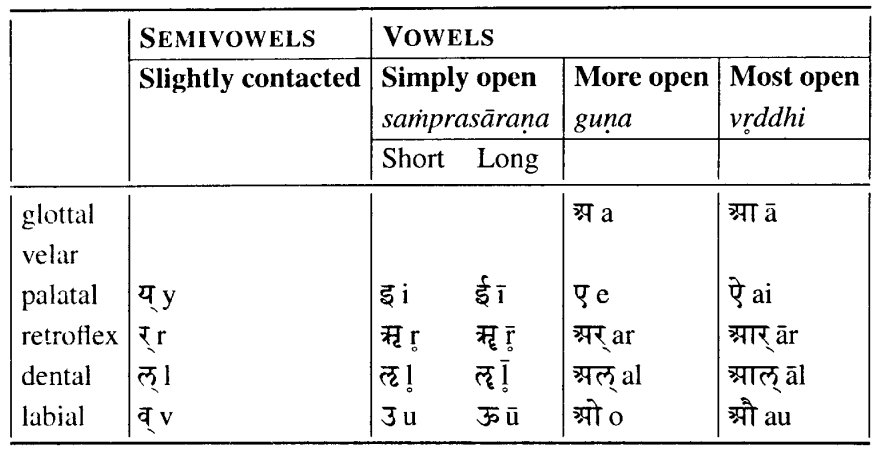
\includegraphics[width=\textwidth]{gunavrddhi.png}
\end{frame}

\begin{frame}{按连声区别}
  %\small
  \centering
  %\resizebox{\textwidth}{!}{
    \begin{tabular}{@{}ccc@{}} % 6 columns
      零级 & 二合 & 三合  \\
      \hline
      \fullpada{ṛ/ṝ}  & \fullpada{ar} & \fullpada{ār}   \\
      \fullpada{ḷ}  & \fullpada{al} & \fullpada{āl}   \\
      \hline
      \fullpada{i/ī} & \fullpada{ay/e} & \fullpada{āy/ai} \\
      \fullpada{u/ū} & \fullpada{av/o} & \fullpada{āv/au} \\
      \hline
      \fullpada{-} & \fullpada{a} & \fullpada{ā} \\
    \end{tabular}
  %}
\end{frame}

\begin{frame}{i和u的历史变化}
  \centering
  \begin{NiceTabular}{@{}cccccc@{}}
    零级 & \Block{1-2}{二合} &   & \Block{1-2}{三合} & & 后音\\
    \Block{2-1}{\fullpada{i/ī}} & \Block{2-1}{\reconstruction{ai}} & \fullpada{e} & \Block{2-1}{\reconstruction{āi}} & \fullpada{ai} & 辅音 \\
                                &                                  & \fullpada{ay} &                                   & \fullpada{āy} & 元音 \\
    \Block{2-1}{\fullpada{u/ū}} & \Block{2-1}{\reconstruction{au}} & \fullpada{o} & \Block{2-1}{\reconstruction{āu}} & \fullpada{au} & 辅音 \\
                                &                                  & \fullpada{av} &                                  & \fullpada{āv} & 元音 \\
  \end{NiceTabular}
\end{frame}

\subsection{应用}

\subsection{~~~现在时语干}
\begin{frame}{\insertsubsection }
  \begin{itemize}
    \item 第一类动词:\verbroot{bhṛ}~\fullpada{bharati}
    
    \notsoimportant{词根元音前加 \nobreakdash-a\nobreakdash-,词根后加 \nobreakdash-a\nobreakdash-。}

    词根二合,后加 \nobreakdash-a\nobreakdash-。
    \item 第四类动词:\verbroot{snih}~\fullpada{snihyati}
      
    \notsoimportant{词根不变,后加 \nobreakdash-ya\nobreakdash-。}

    词根零级,后加 \nobreakdash-ya\nobreakdash-。
    \item 第六类动词:\verbroot{muc}~\fullpada{muñcati}
    
    \notsoimportant{词根不变,后加 \nobreakdash-a\nobreakdash-。}

    词根零级,后加 \nobreakdash-a\nobreakdash-。
  \end{itemize}
\end{frame}

\subsection{~~~第十类动词}
\begin{frame}{\insertsubsection}
  \begin{itemize}
    \item
      词根变哪级都可能,后加 \nobreakdash-aya\nobreakdash-。
    \item 名转动词:保留名词的级别
    
    \verbroot{cint} ~~\verbstem{cintaya} ~~\fullpada{cintayati} ~~\nounstem{cintā}

    \verbroot{kath} ~\verbstem{kathaya} ~\fullpada{kathayati} ~\nounstem{kathā}
    \item 其他:能产生重音节的最低级

    \verbroot{cur} ~~\verbstem{coraya} ~~\fullpada{corayati}

    \verbroot{kṣal} ~\verbstem{kṣālaya} ~\fullpada{kṣālayati}
  \end{itemize}    
\end{frame}

\begin{frame}{补充:轻重音节}
  %\small
  \centering
  \begin{NiceTabular}{@{}ll@{}} % 6 columns
    轻音节 &  短元音 \\
    \\
    重音节 & 长元音、复合元音  \\
     & 后面是复合辅音的短元音 \\
     & 后面带有ṃ或ḥ的短元音 \\
  \end{NiceTabular}
\end{frame}

\subsection{~~~致使动词}
\begin{frame}{\insertsubsection}
  \begin{itemize}
    \item
      其他类的动词按照第十类变化。    
  \end{itemize}
  \centering
  \begin{tabular}{@{}llllll@{}} % 6 columns
      词根 & 现在时 & 致使形式  \\
      \verbroot{viś (6)} & \fullpada{viśati} & \fullpada{veśayati} \\
      \verbroot{dṛś (4)} & \fullpada{paśyati} & \fullpada{darśayati} \\
      \verbroot{bhṛ (1)} & \fullpada{bharati} & \fullpada{bhārayati} \\
    \end{tabular}
  \begin{itemize}
    \item
      以 \nobreakdash-ā 结尾的词根在 \nobreakdash-aya\nobreakdash- 前加 \nobreakdash-p\nobreakdash-。  
  \end{itemize}
  \begin{tabular}{@{}llllll@{}} % 6 columns

      \verbroot{sthā (1)} & \fullpada{tiṣṭhati} & \fullpada{sthāpayati} \\
    \end{tabular}
\end{frame}

\subsection{词根的级别}
\begin{frame}{\insertsubsection }
  \begin{itemize}
    \item
      词根元音一般是零级。 
    \item  有些词根的二合三合是后面加 a/ā
  \end{itemize}
  \centering
  \begin{tabular}{@{}llllll@{}} % 6 columns
      词根 & 现在时 & 零级 & 三合  \\
      \verbroot{yaj (1)} & \fullpada{yajati} & ij & yāj \\
      \verbroot{rakṣ (1)} & \fullpada{rakṣati} & ṛkṣ & rākṣ \\
      \verbroot{vac (2)} & \fullpada{vakti} & uc & vāc \\
      \verbroot{svap (2)} & \fullpada{svapiti} & sup & svāp \\
    \end{tabular}
\end{frame}

\begin{frame}{\insertsubsection }
  \begin{itemize}
    \item  以鼻音结尾的词根
  \end{itemize}
  \centering
  \begin{NiceTabular}{@{}llll@{}} % 6 columns
      词根 & 现在时 & 零级 & 三合  \\
      \Block{2-1}{\verbroot{gam (1)}} & \Block{2-1}{\fullpada{gacchati}} & 元音前gm & \Block{2-1}{gām} \\
                                &                                  & 辅音前ga &                     \\
      \Block{2-1}{\verbroot{man (4)}} & \Block{2-1}{\fullpada{manyate}} & 元音前mn & \Block{2-1}{mān} \\
                                &                                  & 辅音前ma &                     \\
    \end{NiceTabular}
\end{frame}


\section{本节作业}

\begin{frame}{\insertsection }
  \begin{itemize}
    \item
      第七章练习7
    \item
      阅读教材第7课相关内容
    \bigskip
    \item
      现在请做学习通\nobreakdash-章节\nobreakdash-课后问卷
  \end{itemize}
\end{frame}  

\end{document}	
